% \documentclass[11pt]{aghdpl}
\documentclass[en,12pt]{aghdpl}  % praca w języku angielskim

% Lista wszystkich języków stanowiących języki pozycji bibliograficznych użytych w pracy.
% (Zgodnie z zasadami tworzenia bibliografii każda pozycja powinna zostać utworzona zgodnie z zasadami języka, w którym dana publikacja została napisana.)
\usepackage[polish,english]{babel}

% Użyj polskiego łamania wyrazów (zamiast domyślnego angielskiego).
% \usepackage{polski}

\usepackage[utf8]{inputenc}

% dodatkowe pakiety
\usepackage{mathtools}
\usepackage{amsfonts}
\usepackage{amsmath}
\usepackage{amsthm}
\usepackage{hyperref}

% --- < bibliografia > ---

\usepackage[
style=numeric,
sorting=none,
% Zastosuj styl wpisu bibliograficznego właściwy językowi publikacji.
language=autobib,
autolang=other,
% Zapisuj datę dostępu do strony WWW w formacie RRRR-MM-DD.
urldate=iso,
seconds=true,
% Nie dodawaj numerów stron, na których występuje cytowanie.
backref=false,
% Podawaj ISBN.
isbn=true,
% Nie podawaj URL-i, o ile nie jest to konieczne.
url=false,
% Ustawienia związane z polskimi normami dla bibliografii.
maxbibnames=3,
% Jeżeli używamy BibTeXa:
backend=bibtex
]{biblatex}

\usepackage{fvextra}
\usepackage{csquotes}
% Ponieważ `csquotes` nie posiada polskiego stylu, można skorzystać z mocno zbliżonego stylu chorwackiego.
\DeclareQuoteAlias{croatian}{polish}

\addbibresource{bibliography.bib}

% Nie wyświetlaj wybranych pól.
%\AtEveryBibitem{\clearfield{note}}

% Użyj czcionki kroju Courier.
\usepackage{courier}


% ------------------------

\AtBeginDocument{
	\renewcommand{\tablename}{Table}
	\renewcommand{\figurename}{Picture}
}

% ------------------------
% --- < tabele > ---

\usepackage{array}
\usepackage{tabularx}
% \usepackage{slashbox}
\usepackage{diagbox}
\usepackage{multirow}
\usepackage{booktabs}
\usepackage{makecell}
\usepackage[flushleft]{threeparttable}

% defines the X column to use m (\parbox[c]) instead of p (`parbox[t]`)
\newcolumntype{C}[1]{>{\hsize=#1\hsize\centering\arraybackslash}X}

% ------------------------
% --- < glossary > ---

\usepackage[automake, acronyms, toc, nopostdot, nonumberlist, nomain]{glossaries}
\makeglossaries
\loadglsentries{glossaries}
% \glsaddall

% ------------------------
% --- < minted > ---

\usepackage[outputdir=build]{minted}
\usepackage{xcolor}
\definecolor{bg}{rgb}{0.95,0.95,0.95}
\setminted{
  fontfamily=txtt,
  fontsize=\footnotesize,
  samepage=false,
  style=xcode,
  breaklines,
  bgcolor=bg
}
% listings with page breaking
\newenvironment{longlisting}{\captionsetup{type=listing}}{}

% custom lexer for toml
\newminted[tomlcode]{../lexers/toml.py:TomlLexer -x}{}
\newmintinline[tomlcodeinline]{../lexers/toml.py:TomlLexer -x}{}
\newmintedfile[tomlfile]{../lexers/toml.py:TomlLexer -x}{}

% custom lexer for ladr
\newminted[ladrcode]{../lexers/ladr.py:LadrLexer -x}{}
\newmintinline[ladrcodeinline]{../lexers/ladr.py:LadrLexer -x}{}
\newmintedfile[ladrfile]{../lexers/ladr.py:LadrLexer -x}{}

% custom lexer for spass
\newminted[spasscode]{../lexers/spass.py:SpassLexer -x}{}
\newmintinline[spasscodeinline]{../lexers/Spass.py:SpassLexer -x}{}
\newmintedfile[spassfile]{../lexers/spass.py:SpassLexer -x}{}

% custom lexer for tptpt
\newminted[tptpcode]{../lexers/tptp.py:TptpLexer -x}{}
\newmintinline[tptpcodeinline]{../lexers/tptp.py:TptpLexer -x}{}
\newmintedfile[tptpfile]{../lexers/tptp.py:TptpLexer -x}{}
%---------------------------------------------------------------------------

\author{Mateusz Grzeliński}
\shortauthor{M. Grzeliński}

%\titlePL{Przygotowanie bardzo długiej i pasjonującej pracy dyplomowej w~systemie~\LaTeX}
%\titleEN{Preparation of a very long and fascinating bachelor or master thesis in \LaTeX}

\titlePL{System losowego generowania formuł logicznych dla logiki pierwszego rzędu}
\titleEN{System of random generation of logical formulas for first order logic}


\shorttitlePL{Losowy generator formuł logiki pierwszego rzędu}
\shorttitleEN{Random FOL formula generator}

\thesistype{Praca dyplomowa}
\thesistype{Bachelor of Science Thesis}

% \supervisor{dr inż. Radosław Klimek }
\supervisor{Radosław Klimek PhD, DSc}

% \degreeprogramme{Informatyka}
\degreeprogramme{Computer Science}

\date{2020}

% \department{Katedra Informatyki Stosowanej}
% \department{Department of Applied Computer Science}

\faculty{Wydział Elektrotechniki, Automatyki, Informatyki i Inżynierii\protect\\[-1mm]Biomedycznej}
% \faculty{Faculty of Electrical Engineering, Automatics, Computer Science and Biomedical Engineering}

% \acknowledgements{}


\setlength{\cftsecnumwidth}{10mm}

%---------------------------------------------------------------------------
\setcounter{secnumdepth}{4}
\brokenpenalty=10000\relax

\begin{document}

\titlepages

% Ponowne zdefiniowanie stylu `plain`, aby usunąć numer strony z pierwszej strony spisu treści i poszczególnych rozdziałów.
\fancypagestyle{plain}
{
	% Usuń nagłówek i stopkę
	\fancyhf{}
	% Usuń linie.
	\renewcommand{\headrulewidth}{0pt}
	\renewcommand{\footrulewidth}{0pt}
}

\setcounter{tocdepth}{2}
\tableofcontents
\newpage

% \chapter{Abstract}
% This thesis is an implemenetation of random first order logic formula generator. The input of generator describes required formula (number of variables, predicates, clauses and more) and the output is CNF formula encoded in TPTP (Thousands of Problems for Theorem Provers) format. Such formulas can be used to measure performance of SAT solvers what is shown in presented example, as generated dataset is benchmarked against 2 chosen first order logic provers. This dataset represents random system properties.

\chapter{Introduction} \label{cha:Introduction}

\gls{SAT} is the problem of determining if there exists an interpretation that satisfies a given boolean formula. For solving such problem dedicated programs are created, called SAT solvers. Recently there has been substantial development in this area. Modern approach to SAT solving will likely use conflict-driven clause learning \cite{series/faia/SilvaLM09}, various heuristics and make use of better and better hardware. This rapid development in theory of solving SAT problems is followed by number of implementations. Picking best (fastest) implementation of SAT solver for given input problem is not trivial as solving algorithms are based on similar algorithm. Moreover SAT problem has NP complexity what encourages optimizing solvers to specific cases - that is if input formula has frequent pattern, it would be beneficial to optimize solver around that pattern.

SAT problem can be represented in many logical systems and can contain various theories. To name a few possibilities, problem can be expressed with first order logic or propositional logic, additionally integer or floating point arithmetic may be used if needed. The use of appropriate theories must be carefully chosen by engineer when encoding a problem into logical formula as it will affect available range of SAT solver. Having that done, engineer must choose best solver for presented problem. This can be done by benchmarking chosen solver against set of formulas. Pre-generated input formulas can be often obtained from projects like \gls{TPTP} but sometimes custom set of formulas would be handy (see chapter~\ref{chap:Generator} for more detail on available datasets).

This thesis focuses on creating a tool that will assist generating custom set of formulas. The basic function of this tool is generating random set of formulas which can be used to test performance of solvers. 
The goal is to create extendable, easy to use \gls{FOL} formula generator.
Generator has this advantage over pre-generated dataset that it can precisely map encountered real-life problem into measurable, repeatable custom dataset. It is important for the ease of use to keep inner representation of first order logic the same as mathematical definitions of elements of first order logic. Any arbitrary rule can be injected into generation to fulfill user specific needs. Those rules are meant to represent fragment or reality that engineer wants to represent in \gls{FOL}. Formulas generated in this way can be used as testing tool as randomness of formulas can be finely controlled. 
First order logic has been chosen deliberately. First order logic can be considered well balanced then it comes to expressiveness, complexity and adaptation among solvers. Less expressive and simpler logic would be propositional logic, whereas more complex logic is for example higher order logic. 


\chapter{Logical systems}
% https://en.wikipedia.org/wiki/Mathematical_logic#Formal_logical_systems
% https://en.wikipedia.org/wiki/Formal_system#Logical_system
% https://en.wikipedia.org/wiki/Formal_system
% https://cs.lmu.edu/~ray/notes/formalsystems/
% https://en.wikipedia.org/wiki/Formal_system
% https://cs.lmu.edu/~ray/notes/formalsystems/

Formulas must be presented in some kind of formal system. A formal system consists of a language over some alphabet of symbols together with (axioms and) inference rules that distinguish some of the strings in the language as theorems. These rules used to carry out the inference of theorems from axioms are known as the logical calculus of the formal system. A formal system may represent a well-defined system of abstract thought. A logical system is a formal system together with its semantics. Some recognizable logical formal systems are:

\begin{itemize}
  \item propositional logic 
  \item first order logic (FOL)
  \item higher order logic (HOL)
  \item temporal logic 
\end{itemize}

The majority of formulas are probably going to be represented in propositional calculus because of simplicity of such notation. Propositional logic deals with variables which are connected with logical connectives. Variable can be true or false. Formula in propositional logic is easy to parse but may become quite long when compared to different formal logical systems. For more complex problem it may be easier to encode problem in more expressive system and the next natural step would be first order logic as it is not redefinition but extension of propositional logic.

\section{First Order Logic}

First order logic (also known as predicates logic, first-order predicate calculus) extends propositional logic by adding predicates, functors and quantifiers and non-logical objects. Definitions of FOL elements are contained below.

% http://mathworld.wolfram.com/First-OrderLogic.html
\textbf{Variable}
unlike propositional logic, variables in \gls{FOL} can stand for a relation (between terms) but which has not been specifically assigned any particular relation.
Usually starts with capital letter. If variables is used in quantifier it is called bound variable, otherwise it is called free variable.

\textbf{Singleton variable}
is used only once in clause.

\textbf{Functor}
is logical operator, that returns term. Functor has constant arity. Usually noted as $functor\_name/arity$, eg. $f/1$. Name of functor  is usually lowercase $f, g, h$.

\textbf{Constant functor}
is functor with arity 0.

\textbf{Predicates}
is logical operator which returns true or false. Predicates operates on specific number of terms. This number is constant and called predicate \textbf{arity}. Usually noted as $predicate\_name/arity$, for example $p/1$. Name of predicate is usually lowercase $p, q, r$. Predicate describes relation between objects.

\textbf{Term}
is variable, constant or result of functor.

\textbf{Atom}
is logical statement, that can not be further divided. Atom consists of predicate, or in case of atom with equality it consists of terms.

\textbf{Literal}
is atom or its negation.

\textbf{Clause}
is disjunction of literals.

\textbf{Unit clause}
is clause with only one literal.

\textbf{Horn clause}
is clause, which contains at least one positive literal.

% https://en.wikipedia.org/wiki/Quantifier_(logic)
\textbf{Quantifier}
specifies the quantity of specimens in the universe that satisfy an open formula (formula with at least one free variable). A formula beginning with a quantifier is called a quantified formula.

\textbf{Existential quantifier}
is equivalent to a logical disjunction of propositions, this is, at least one proposition must be true.

\textbf{Universal quantifier}
is equivalent to a logical conjunction of propositions, this is, all propositions must be true.

The following \gls{FOL} example contains 1 existential quantifier, 2 variables $W$, $Z$, 1 predicate $p/2$, 2 constant functors $a/0$, $b/0$.
\begin{equation} \label{eg:FOL_1}
  \exists_{W,Z} p(W,Z) \lor p(a, b)
\end{equation}

\section{Normal forms}

Representing logic formula in one of normal forms sometimes can enable new or shorter reasoning not available otherwise. One of normal forms mentioned in this thesis is \textbf{conjunctive normal form (CNF)}. It is a conjunction of one or more clauses, where a clause is a disjunction of literals. Other example of normal form is \gls{DNF} where formula is disjunction of conjunctions.

The focus of this thesis is conjunctive normal form as it is one of the most basic forms that represent logical formulas and any statement in \gls{FOL} can be converted to CNF.

\section{Formats used for representing formulas}

There are many formats that allow representing logic, a few of them are described in this section. Many provers implement its own language for representing logic formulas like prover9\footnote{Prover9 is an automated theorem prover for first-order and equational logic \cite{prover9-mace4}} what creates technical problems of comparability between solvers. In this thesis a standard called \gls{TPTP} will be used to represent first order logic formulas.

\subsection{DIMACS}

DIMACS\footnote{\url{https://www.domagoj-babic.com/uploads/ResearchProjects/Spear/dimacs-cnf.pdf}} is also the name of one of popular formats for encoding propositional logic. Although variations of DIMACS can be found, it is mainly used to encode CNF what will be presented next. At the beginning there is always problem line:
\mintinline{text}{p cnf VARIABLES CLAUSES},
where VARIABLES is number of variables in formula and CLAUSES is number of clauses in formula. $c$ means line is a comment. Variables are noted with integers, negation is minus sign. Clause delimiter is 
\mintinline{text}{0}. 

\begin{listing}[H]
\begin{minted}{text}
p cnf 3 2
1 -3 0
2 3 -1 0
\end{minted}
  \caption{DIMACS formula example, formula consists of 2 clauses, 3 variables ($1$, $2$, $3$) and 5 literals)}
  \label{lis:DIMACSExample}
\end{listing}

\subsection{SMT-LIB}

SMT-LIB \cite{BarFT-RR-17} is an international initiative aimed at facilitating research and development in \gls{SMT}. Its 2 major projects handled by SMT-LIB are defining standard for encoding logical problems and creating benchmarks (more about benchmarks in section \ref{sec:SMTLIBBenchmarks}). Mentioned standard covers:

\begin{itemize}
  \item a language for writing terms and formulas in a version of first order logic - it means that using SMT-LIB any subset of first order logic can be presented, including propositional logic
  \item a language for specifying background theories and defining a standard vocabulary of symbols for them - it means that theories like integers, floating points, real number etc. can be used. New theories can be easily defined.
  \item a language for specifying logics - it means that new (different than first order logic) logic systems can be created. For example first logic system can allow quantified formulas, second can be quantifier free.
  \item a command language for interacting with SMT solvers - it means in there are syntax elements which allow asserting and retracting formulas, querying about their satisfiability or their unsatisfiability proofs, and so on.
\end{itemize}

Compared to DIMACS, SMT-LIB is much more sophisticated, what can be advantage or disadvantage depending on use case. 

\begin{listing}[H]
  \caption{Example of quantifier free boolean formula with free (uninterpreted) sort and function symbols - QF\_UF}
  \label{lis:SMTLIBExample}
  \begin{minted}{text}
; Basic Boolean example
(set-option :print-success false)
(set-logic QF_UF)
(declare-const p Bool)
(assert (and p (not p))) 
(check-sat) ; returns 'unsat'
(exit)
  \end{minted}
\end{listing}

\subsection{Thousands of Problems for Theorem Provers}
\label{sub:TPTP}

TPTP \cite{Sut17} - Thousands of Problems for Theorem Provers - is both problem library used for testing \gls{ATP} systems and standard describing syntax for those tests. Next to TPTP library there is \gls{TSTP} - library of solutions produced by various solvers. Problems are classified into different domains: LCL - Logic Calculi, COL - Combinatory Logic and more.

TPTP defines syntax for several logic systems: \gls{TPI}, \gls{THF}, \gls{TFF}, \gls{FOF}, \gls{CNF} but in this thesis only \gls{FOF} and \gls{CNF} will be used.

\subsubsection{First order logic in Thousands of Problems for Theorem Provers syntax}

The following description is a description of \gls{FOL} syntax elements used in \gls{TPTP} \footnote{Full technical document for TPTP syntax can be found at \url{http://www.tptp.org/TPTP/TR/TPTPTR.shtml}}.

Variables start with upper case letters, atoms and terms are written in prefix notation, uninterpreted predicates and functors either start with lower case and contain alphanumerics and underscore, or are in 'single quotes'.

Each logical formula is wrapped in an annotated formula structure of the form \mintinline{text}{fof(name,role,formula,source,[useful_info])} or \mintinline{text}{cnf(name,role,formula,source,[useful_info])}

\begin{itemize}
  \item \mintinline{text}{name} is only for documenting purposes
  \item \mintinline{text}{role} gives the user semantics of the formula, in context of SAT problem it will be usually \mintinline{text}{axiom}, but can also for example \mintinline{text}{hypothesis} or \mintinline{text}{definition}. They are accepted, without proof, as a basis for proving conjectures. In CNF problems the axiom-like formulae are accepted as part of the set whose satisfiability has to be established. A problem is solved only when all formulas with role \mintinline{text}{conjecture} are proven. TPTP problems never contain more than one conjecture. \mintinline{text}{negated_conjectures} are formed from negation of a \mintinline{text}{conjecture}, typically in FOF to CNF conversion.
  \item \mintinline{text}{formula} is logical formula
  \item the \mintinline{text}{source} field is used to record where the annotated formula came from, and is most commonly a file record or an inference record
  \item the \mintinline{text}{useful_info} field of an annotated formula is optional, and if it is not used then the \mintinline{text}{source} field becomes optional
\end{itemize}

The language also supports interpreted predicates and functors. These come in two varieties: 
\begin{itemize}
  \item defined predicates and functors, whose interpretation is specified by the TPTP language like \mintinline{text}{$true} and \mintinline{text}{$false}, \mintinline{text}{=} and \mintinline{text}{!=} and arithmetic predicates
  \item system predicates and functors, whose interpretation is \gls{ATP} system specific, like \mintinline{text}{$o} - the Boolean type, \mintinline{text}{$i} - the type of individuals, \mintinline{text}{$real} - the type of reals, \mintinline{text}{$rat} - the type of rational, and \mintinline{text}{$int} - the type of integers.
\end{itemize}

The universal quantifier is \mintinline{text}{!}, the existential quantifier is \mintinline{text}{?}, and the lambda binder is \mintinline{text}{^}. Quantified formulae are written in the form \mintinline{text}{Quantifier [Variables] :  Formula}

The binary connectives are infix \mintinline{text}{|} for disjunction, infix \mintinline{text}{&} for conjunction, infix \mintinline{text}{<=>} for equivalence, infix \mintinline{text}{=>} for implication, infix \mintinline{text}{<=} for reverse implication, infix \mintinline{text}{<~>} for non-equivalence (XOR), infix \mintinline{text}{~|} for negated disjunction (NOR), infix	\mintinline{text}{~&} for negated conjunction (NAND), infix \mintinline{text}{@} for application. The only unary connective is prefix \mintinline{text}{~} for negation

\subsubsection{Additional tools in TPTP library}
\label{sub:AdditionalToolsInTPTPLibrary}

TPTP ships with \gls{TPTP4X} (written in c), \gls{TPTP2X} (written in prolog) utilities, which are used for reformatting, transforming, and generating TPTP problem files. Example of functionalities:

\begin{itemize}
  \item converting \gls{FOF} to \gls{CNF} (for example with otter \cite{McC-Otter-URL}, bundy \cite{Bun83} algorithm, details in \cite{SM96})
  \item converting TPTP to syntax required by prover9, dimacs, otter, dfg and more
  \item optimization \gls{FOF}, \gls{CNF} with different algorithms
  \item change order of \gls{CNF}
\end{itemize}

\subsubsection{Examples of FOL and CNF in TPTP syntax}

For comparison examples of \gls{FOL} formulas are also shown in CNF. 

\begin{listing}[H]
  \caption{TPTP FOL formula with existential quantifier, translated to CNF}
\begin{tptpcode}
fof(simple_exists, axiom,
 ? [W,Z] : p(W, Z) | p(a, b)
  ).
% equivalent in CNF, converted with TPTP2X, otter algorithm
cnf(simple_exists_1,axiom,
    ( p(sk1,sk2) | p(a,b) )).
\end{tptpcode}
\end{listing}

\begin{listing}[H]
  \caption{TPTP FOL formula with universal quantifier, translated to CNF}
\begin{tptpcode}
fof(simple_for_all, axiom,
 ! [W,Z] : p(W, Z) | p(a, b)
  ).
% equivalent in CNF, converted with TPTP2X, otter algorithm
cnf(simple_for_all_1,axiom,
    ( p(A,B) | p(a,b) )).
\end{tptpcode}
\end{listing}

\begin{listing}[H]
  \caption{TPTP FOL formula, translated to CNF}
\begin{tptpcode}
% for every X, Y operation lesseq is the same as less or equal
fof(this_is_obvious, axiom,
  ! [X,Y] : ( $lesseq(X,Y) <=> ( $less(X,Y) | X = Y ) )
  ).
% equivalent in CNF, converted with TPTP2X, otter algorithm
cnf(this_is_obvious_1,axiom,
    ( ~ $lesseq(A,B) | $less(A,B) | A = B )).

cnf(this_is_obvious_2,axiom,
    ( ~ $less(A,B) | $lesseq(A,B) )).

cnf(this_is_obvious_3,axiom,
    ( A != B | $lesseq(A,B) )).
\end{tptpcode}
\end{listing}


\chapter{Generator}
\label{chap:Generator}

There are number solutions that provide formulas in a way of generators or benchmarks:

\begin{itemize}
  \item SMT-LIB \cite{BarFT-RR-17} -- is project aimed at facilitating research and development in \gls{SMT} . One part of their activity is defining syntax for representing formulas in with various theories and hosting considerable benchmark library
  \item SATLIB \cite{Hol00} -- is collection of benchmarks of propositional logic (DIMACS CNF format)
  \item Tough SAT \cite{ToughSAT} -- is a platform that will generate boolean CNF formulas that encode "difficult" problems. Problems are represented in propositional logic (DIMACS CNF format). Although Tough SAT is in fact generator it supports only several predefined problems like Factoring, Subset Sum, Random k-SAT, Cocktail.
% \item PySAT\footnote{\url{https://pysathq.github.io/}} -- is a toolkit, which aims at providing a simple and unified interface to a number of SAT solvers as well as to a variety pseudo-Boolean encodings. Rather than generating benchmarks this tool is useful when there is a need to access several solvers with unified interface.
  \item CNFgen \cite{CNFGen} -- produces combinatorial benchmarks in DIMACS format. These benchmarks come mostly from research in Proof Complexity (pigeonhole principle, ordering principle, k-clique and more). Many of these formulas encode structured combinatorial problems well known to be challenging for certain SAT solvers.
  \item \gls{TSTP} (Thousands of Solutions from Theorem Provers) a side project of \gls{TPTP} \cite{Sut17} -- it is a library of problems and solutions encoded in TPTP format
\end{itemize}

Although a lot of ready to use benchmarks can be found, there are not a lot of generators. Tough SAT and CNFgen are generators that generate predefined problem with given size, SMT-LIB, SATLIB, TSTP are mainly repositories of benchmarks, not generators itself. Out of mentioned solutions only SMT-LIB and TSTP support first order logic. None of mentioned solutions can generate first order logic formulas. 

A random first order formula would be useful in this sense, that it would allow creating new datasets with precisely controlled elements. A parameters for such generator shall be described next.

\newpage

\section{Defining CNF Generator}

User defines generator in 2 steps:

\begin{enumerate}
  \item General setting for generated formula

    In this step user defines set of allowed \gls{FOL} elements:
    \begin{itemize}
      \item set of variable names $\{'v1','v2',\dots\}$
      \item set of functor names $\{'f1','f2',\dots\}$
      \item set of predicate names $\{'p1','p2',\dots\}$
      \item set of allowed functor arities $a_f = \{0, 1, 2,\dots\}$
      \item maximum recursion depth $n$ for functors
      \item set of allowed predicate arities $a_p = \{0, 1, 2,\dots\}$
      \item set of atom allowed connectives, that is no connective or/and any subset of $AllowedConnectives = \{=, !=, \emptyset\}$
      \item set of allowed clause lengths $AllowedClausesLengths = \{1,2,\dots\}$
      \item amount of literals to be negated
    \end{itemize}

  \item How many instances of elements are allowed

    In this step user defines what properties formula should have:
    \begin{itemize}
      \item formula contains from $c_{min}$ to $c_{max}$ clauses
      \item formula contains from $l_{min}$ to $l_{max}$ literals
    \end{itemize}
\end{enumerate}

Basic algorithm of generating formula consists of following steps:

\begin{enumerate}
  \item Resolve user constraints~\ref{sec:ResolveUserConstrains}
  \item Generate possible formula based on generators~\ref{sec:Generators}
  \item Generate statistics and export formula to file~\ref{sec:GenerateStatisticsAboutFormula}
\end{enumerate}


\section{Resolve user constraints}
\label{sec:ResolveUserConstrains}

User constrains are defined in input parameters as $AllowedClausesLengths$, $NumberOfClauses$, $NumberOfLiterals$. To generate random formula withing these constrains, number of clauses with appropriate clause length must be computed.

CNF formula $F_{cnf}$ consists of unordered clauses $c1, c2, \dots$. 

\begin{align*}
	&F_{cnf}(x) = \{c1, c2, \dots\, cx\} \\
	\text{where }
		&x \text{ -- number of clauses in formula}
\end{align*}

If we group clauses by their length:
\begin{align*}
	&F_{cnf}(x) = \bigcup_{i=1}^c c_i \\
	\text{where }
		&c_i \text{ -- set of clauses with length i} 
\end{align*}

Number of literals in formula can be represented as:
\begin{align*}
	l(x) &= x_1|c_1| + x_2|c_2| + \dots + x_x|c_x| = \sum_{i=1}^{x} x_i |c_i| \\
	x &= x_1 + x_2 + \dots + x_n \\
	c_i &\in AllowedClausesLen: \forall_{i \neq j} c_i \neq c_j  \\
	\text{where }
		&x \text{ -- number of clauses in formula} \\ 
		&l(x) \text{ -- number of literals in formula} \\ 
		&|c_i| \text{ -- number of clauses with length i} 
\end{align*}

So in the end:

\begin{align}
  l(x) &= \sum_{i=1}^{x} x_i |c_i|\label{eq:UserConstraintsLx} \\
  x &= \sum_i^x x_i\label{eq:UserConstraintsX} \\
  l_{min} &< l(x) < l_{max} \label{eq:UserConstraintsRangeL}\\
  c_{min} &< x < c_{max}\label{eq:UserConstraintsRangeC} \\
	\text{where } 
		&x \text{ -- number of clauses in formula} \nonumber \\
		&l(x) \text{ -- number of literals in formula} \nonumber  \\
		&|c_i| \text{ -- number of clauses with length i} \nonumber
\end{align}

Solution of above equation are pairs of numbers: clause length and how many clauses with this length should be used in generated clause.

\subsection{Using Z3 to resolve user constraints}

Z3 \cite{Z3Solver} is a \gls{SMT} prover from Microsoft Research. It uses SMT-LIB as input format, but also has bindings to multiple languages. It can be used to solve user constraints presented in~\ref{sec:ResolveUserConstrains}. Z3 supports arithmetic what is essential for solving user constraints.

Solving equation is implemented as class $CNFConstraintSolver$ (picture~\ref{pic:ConstraintSolverZ3ClassDiagram}). Parameter $allowed\_clause\_lengths$ corresponds to $c_i$ in equation~\ref{eq:UserConstraintsLx}, parameter $number\_of\_literals$ corresponds range of allowed values of literals - tuple of minimal and maximum range - ($l(x)$ in equation~\ref{eq:UserConstraintsLx}), parameter $number\_of\_clauses$ corresponds number of allowed values of clause - tuple of minimal and maximum range - ($x$ in equation~\ref{eq:UserConstraintsX}). The set of variables $x_i$ will be returned from method $solve()$ as dictionary, where key is $i$ (clause length) and value is how many clauses are needed.


\begin{figure}[h]
\begin{centering}
  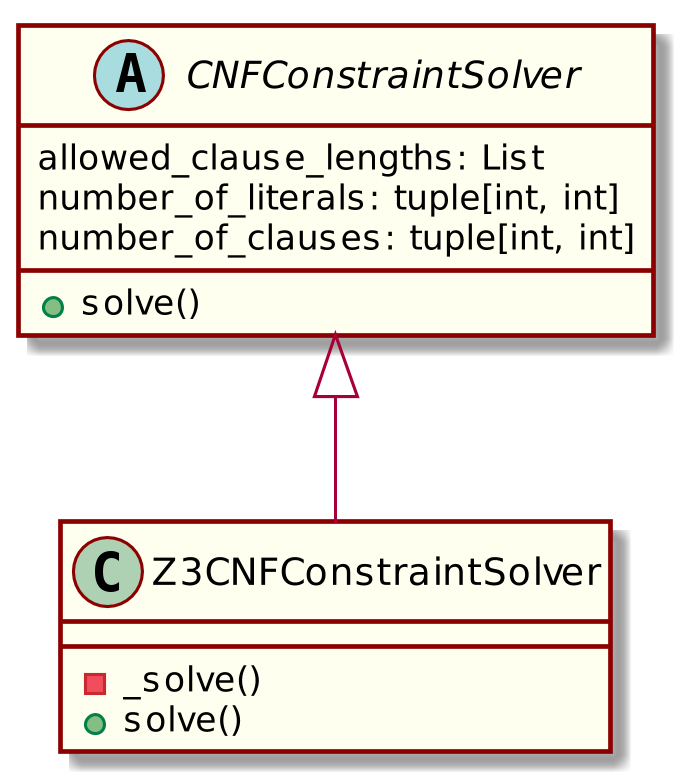
\includegraphics[width=0.3\textwidth]{logic-formula-generator/fol/resolve_constraints.png}
  \caption{Subclassed constraint solver}
  \label{pic:ConstraintSolverZ3ClassDiagram}
\end{centering}
\end{figure}

Function \mintinline{text}{_solve()} in listing \ref{lis:DeterministicSolve} solves user constraints using Z3 solver bindings in Python. Line 
\mintinline{python}{X = [z3.Int() ...]}
defines Z3 variables, which can contain only integer values. This variable is used to represent $x_i$ from \ref{eq:UserConstraintsX}. Further down the line 
\mintinline{python}{s = z3.Solver()} 
creates model, to which constraints will be added. Constraints are defined by functions
\mintinline{python}{z3.Sum}, 
\mintinline{python}{z3.And}, 
and can be added to model via
\mintinline{python}{s.add}.
Variables must follow 2 rules: they must be non negative and be in range defined by \ref{eq:UserConstraintsRangeC} and \ref{eq:UserConstraintsRangeL}. Solution can be calculated from model with 2 operations: first check if model is satisfayable, next evalueate (get value) of variables in model. If another solution is needed, it can be done by adding constraints, that forbids concurrencyent solution and recalculating model.


\begin{listing}[H]
  \caption{Lazy, deterministic function for solving user constraints}
  \label{lis:DeterministicSolve}
\begin{minted}{python}
    def _solve(self) -> Iterable[Dict[int, int]]:
        """Solve in deterministic order"""
        A = self.literal_coefficients
        n = len(A)
        X = [z3.Int() for i in range(n)]
        s = z3.Solver()

        # solutions must be positive
        s.add(z3.And([X[i] >= 0 for i in range(n)]))

        # clauses must be in range
        s.add(z3.Sum(X) <= self.number_of_clauses[1])
        s.add(z3.Sum(X) >= self.number_of_clauses[0])

        # literals must be in range
        s.add(z3.Sum([A[j] * X[j] for j in range(n)]) <= self.number_of_literals[1])
        s.add(z3.Sum([A[j] * X[j] for j in range(n)]) >= self.number_of_literals[0])

        while s.check() == z3.sat:
            solution = [s.model().evaluate(X[i]) for i in range(n)]
            yield {clause_len: s.as_long() for clause_len, s in zip(A, solution)}
            forbid = z3.Or([X[i] != solution[i] for i in range(n)])
            s.add(forbid)
\end{minted}
\end{listing}

Fundamental problem of using SAT (or SMT) solver in this scenario when any, random solution is needed, is fact that solver will always produce deterministic result for the same input data. There are 2 solutions for this problem. First one, presented here, is using a wrapper that will temporarily skip or discard part of solutions, to randomize deterministic output. In this cave, non public function $\_solve$ in listing~\ref{lis:DeterministicSolve} is a function that actually yields solutions and $solve$ in listing \ref{lis:RandomSolve} is a randomizing wrapper. Randomization occurs at the cost of time and memory. Second approach assumes that solver supports soft clause\footnote{contrary to hard clauses, soft clauses does not have to be satisfied}. Using soft clauses a random starting point can be suggested to a solver. For example line added to listing \ref{lis:DeterministicSolve} \mintinline{python}{s.add(z3.Sum([A[j] * X[j] for j in range(n)]) == random_number))} would hint Z3 solver to strat in \mintinline{text}{random_number} if Z3 supported this feature in Python bindings.

\begin{listing}[H]
  \caption{Lazy, randomizing wrapper around deterministic solver~\ref{lis:DeterministicSolve}}
  \label{lis:RandomSolve}
\begin{minted}{python}
    def solve(self, skip_chance: float = None):
        """Solve in random order"""
        skip_chance = random.random() if skip_chance is None else skip_chance
        cache = []
        for solution in self.solve():
            if random.random() < skip_chance:
                yield solution
            else:
                cache.append(solution)

        random.shuffle(cache)
        for cached_solution in cache:
            yield cached_solution
\end{minted}
\end{listing}

\section{Intermediate representation}

Abstract syntax tree of \gls{FOL} is implemented in the same way as mathematical definition, see picture~\ref{pic:fol_elements_class_diagram}. All classes have base class $FolElement$ so that they can be easily identified as element of first order logic and introduce visitor pattern. Visitor pattern is used for exporting formula from intermediate representation to the format of choice (like \gls{TPTP}) as well as counting statistics about generated formula. See for example listing~\ref{lis:TPTPExample} - it is convention from TPTP to store some statistics about file at the beginning of file as comment.

Variable and functor are terms, that is why the inherit from term class. Functor is recursive structure it can contain variable or another term, that is why it is connected with aggregation with term class. Predicate can contain only terms, atom can contain term or predicate, literal can contain only one atom but adds sign to it, clause is one or more literal, CNF formula is one or more clause.

\begin{figure}[h]
\begin{centering}
  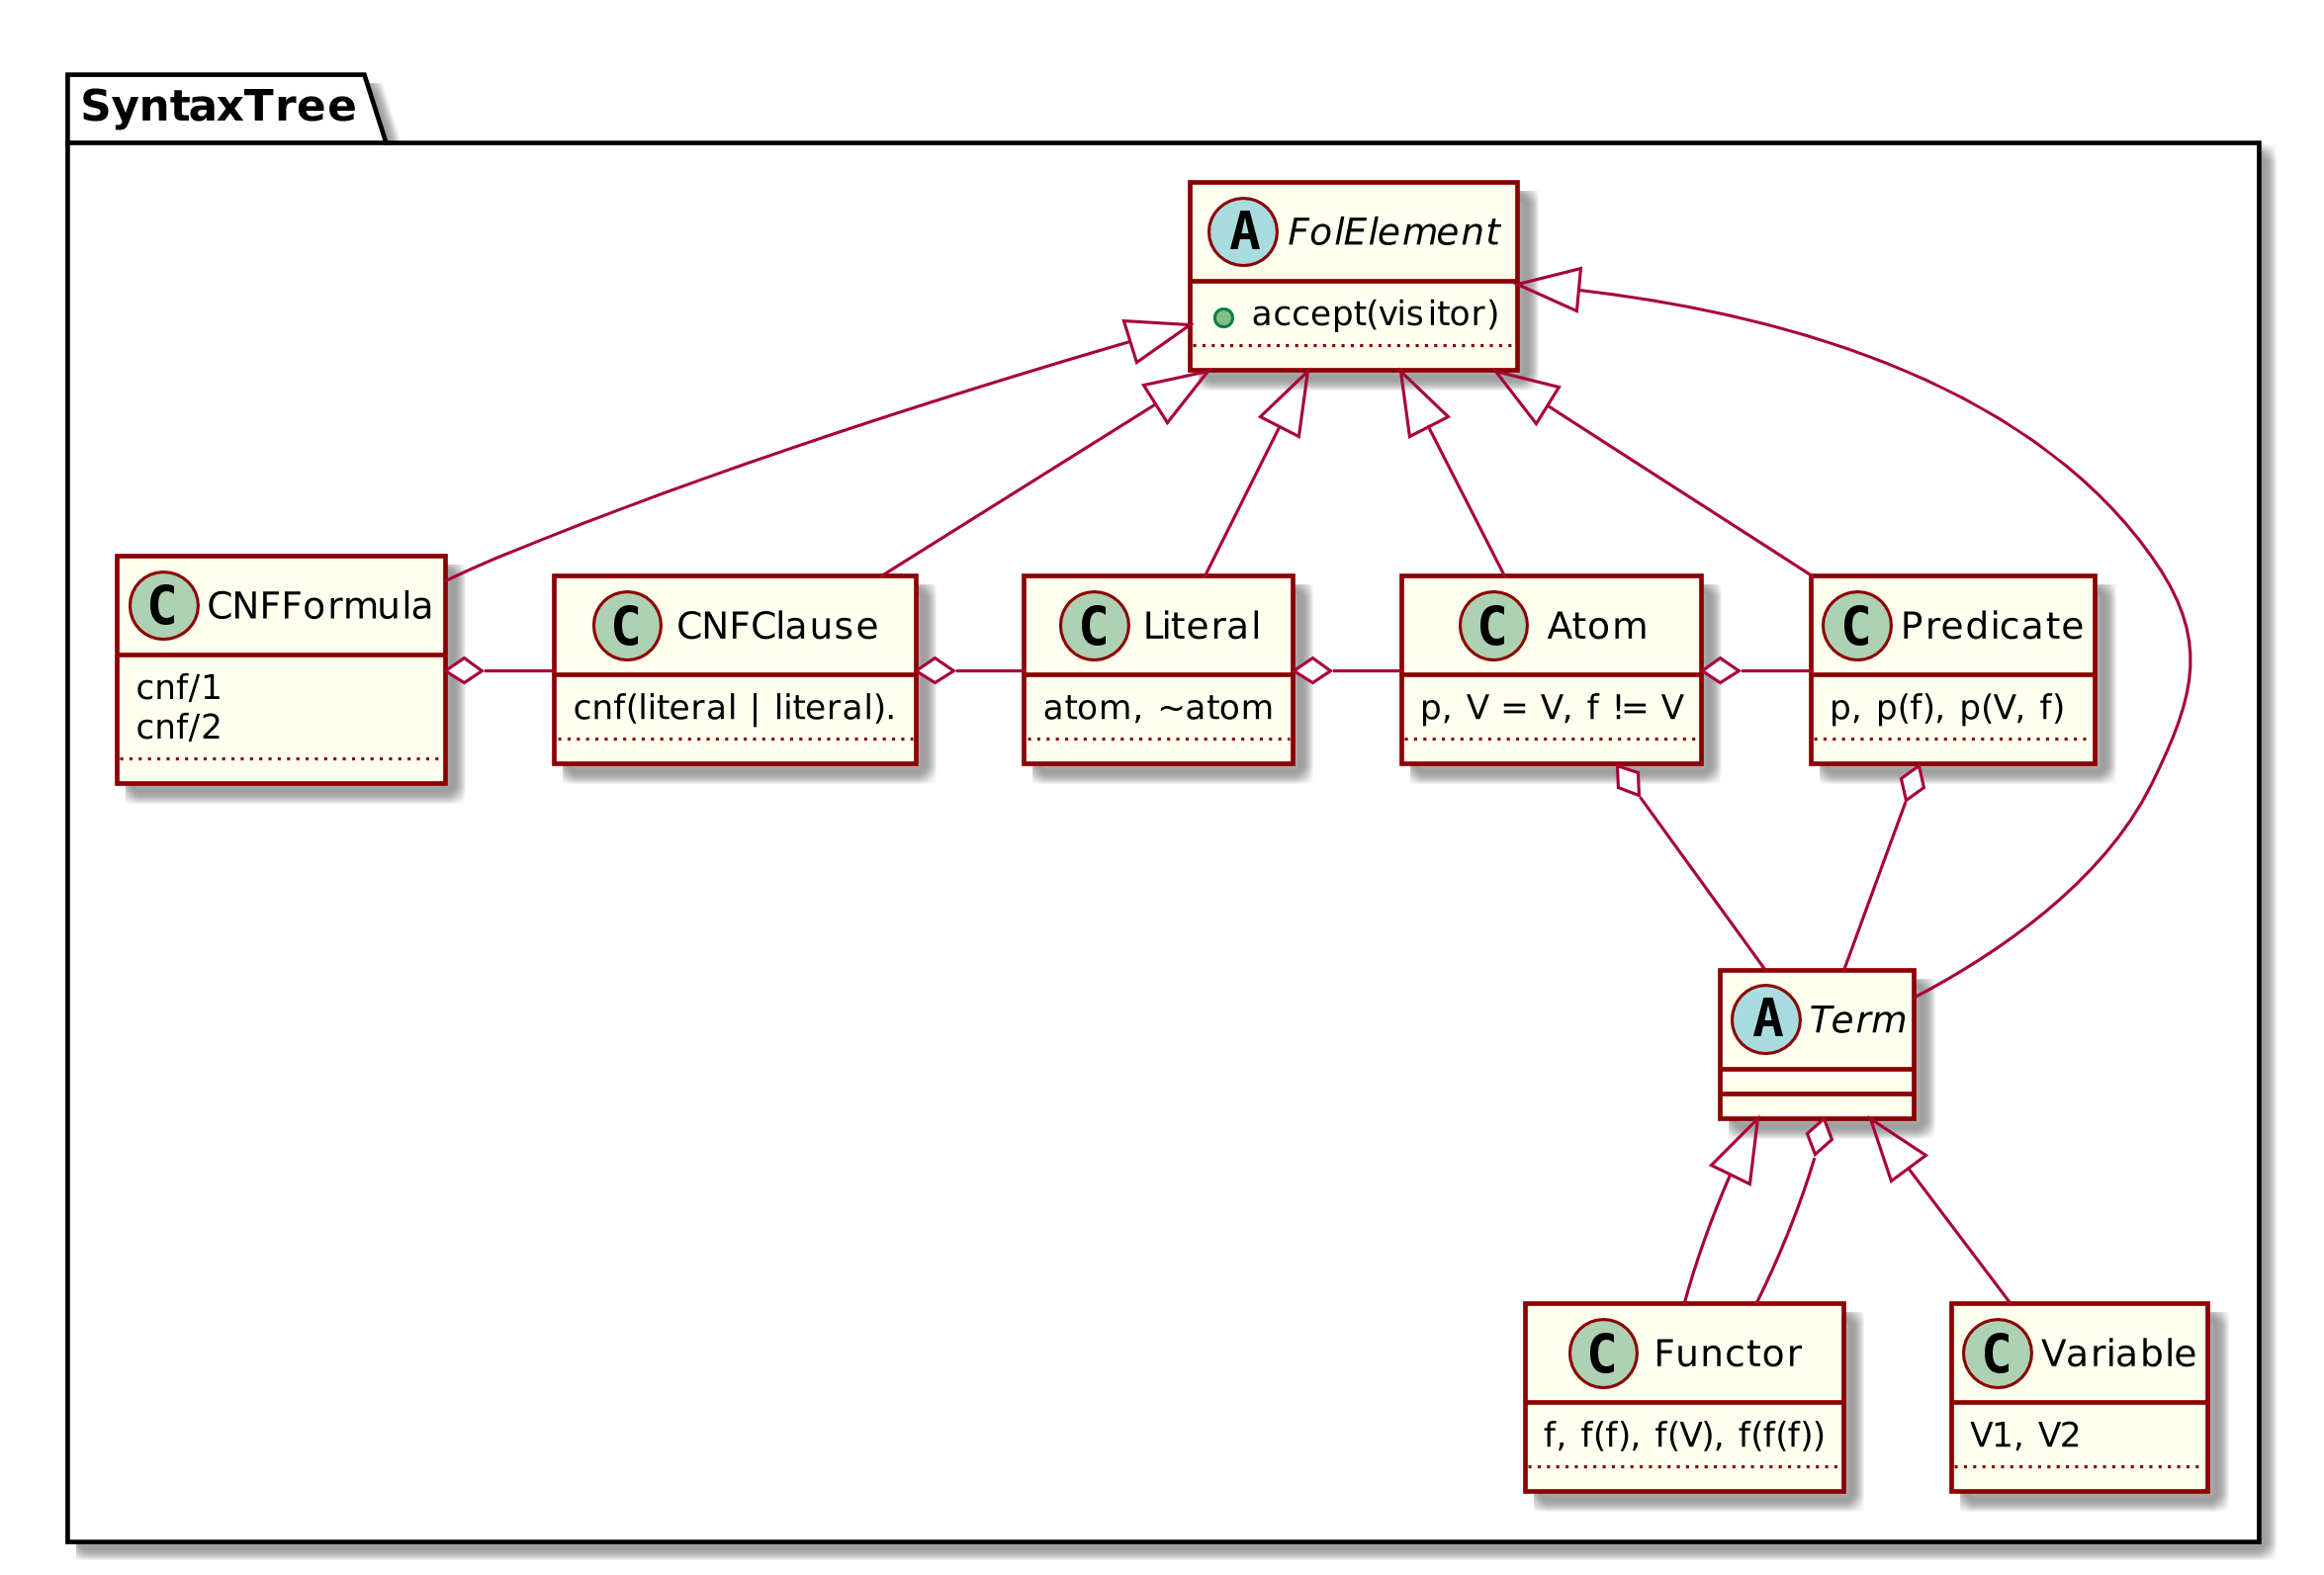
\includegraphics[width=\textwidth]{logic-formula-generator/fol/cnf_fol_elements.png}
  \caption{Class diagram for internal representation of first order logic elements}
  \label{pic:fol_elements_class_diagram}
\end{centering}
\end{figure}

\section{Intermediate representation generators}
\label{sec:Generators}

Generators are implemented as cascade (picture~\ref{pic:fol_signature_generator_class_diagram}), that is formula generator provides formulas, but requires clause generator, clause generator provides clauses, but requires literal generator and so on.

\begin{figure}[h]
\begin{centering}
  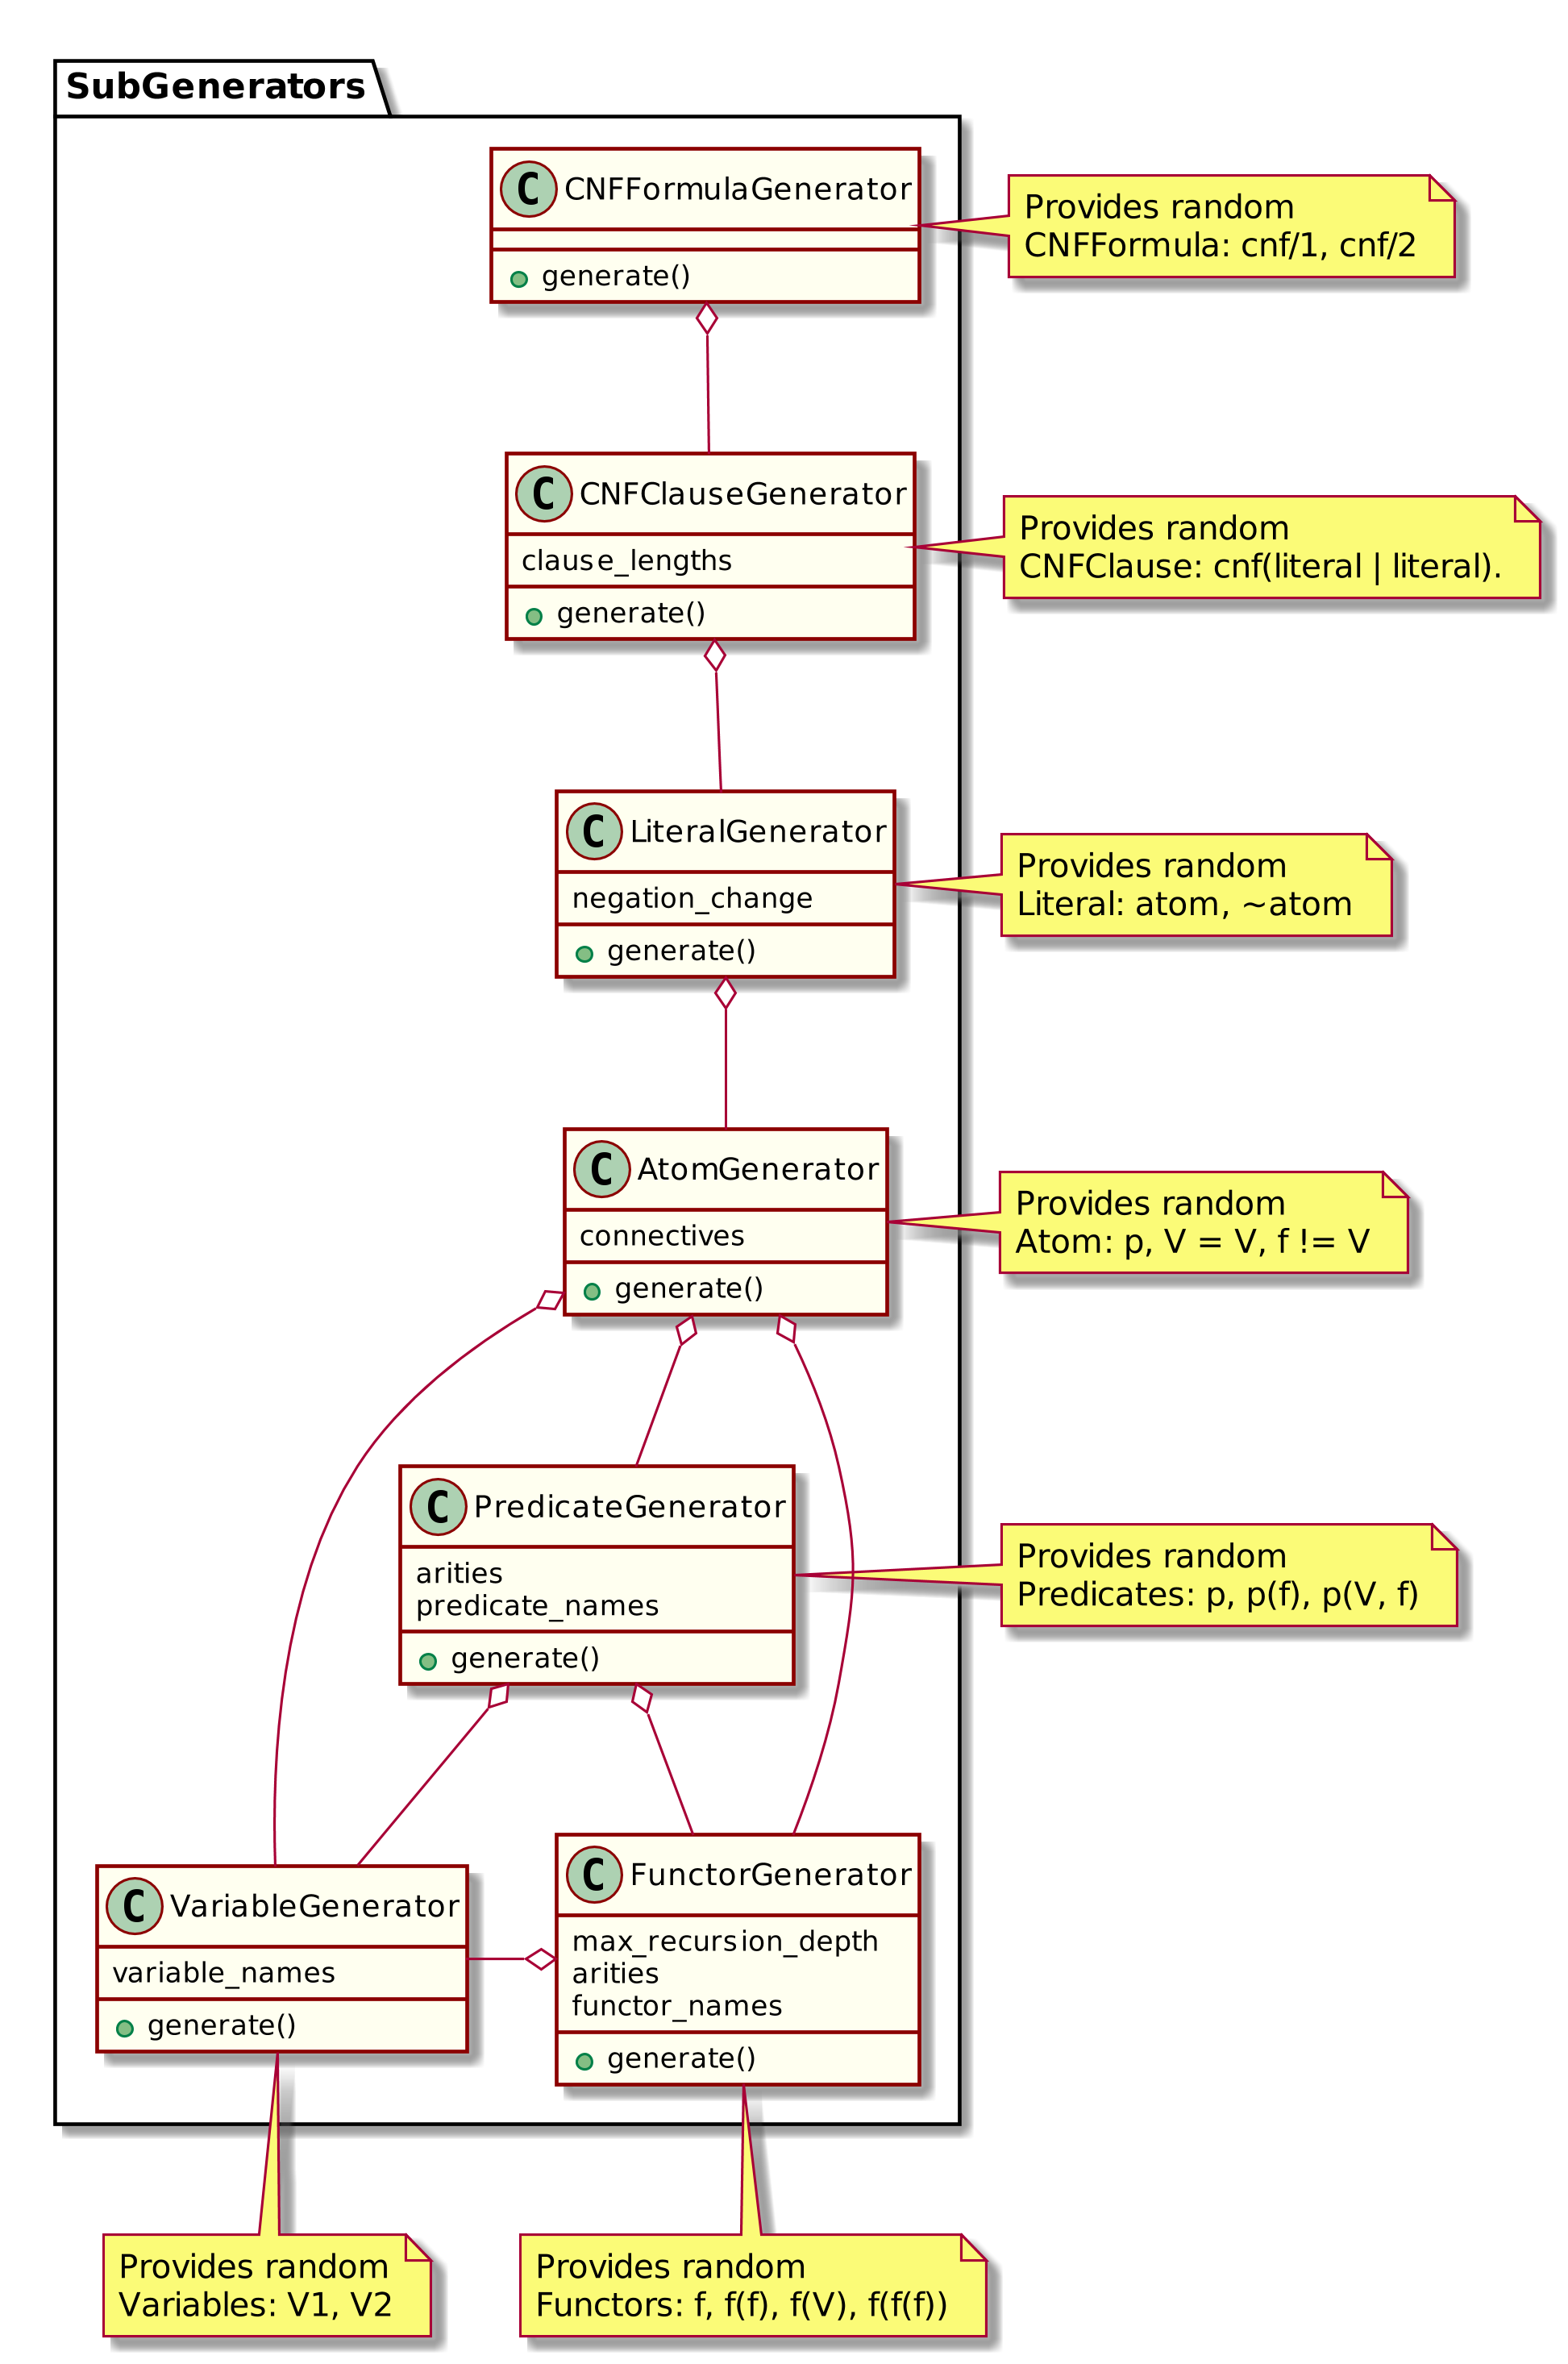
\includegraphics[width=0.7\textwidth]{logic-formula-generator/fol/cnf_signature_generators.png}
  \caption{Class diagram of generators in CNF formula generator}
  \label{pic:fol_signature_generator_class_diagram}
\end{centering}
\end{figure}

Manual creation of generators is required only in advanced case. To automate this process $CNFFormulaGenerator$ (picture~\ref{pic:cnf_generator_class_diagram}) has been created. This is interface for user to create random CNF formulas that will automatically resolve user constraints and yield random formula. After creating formula from signature generators formula will be post processed - given random names and optionally negation sign. Generated formula can be then exported to file along with statistics about formula.

\begin{figure}[h]
\begin{centering}
  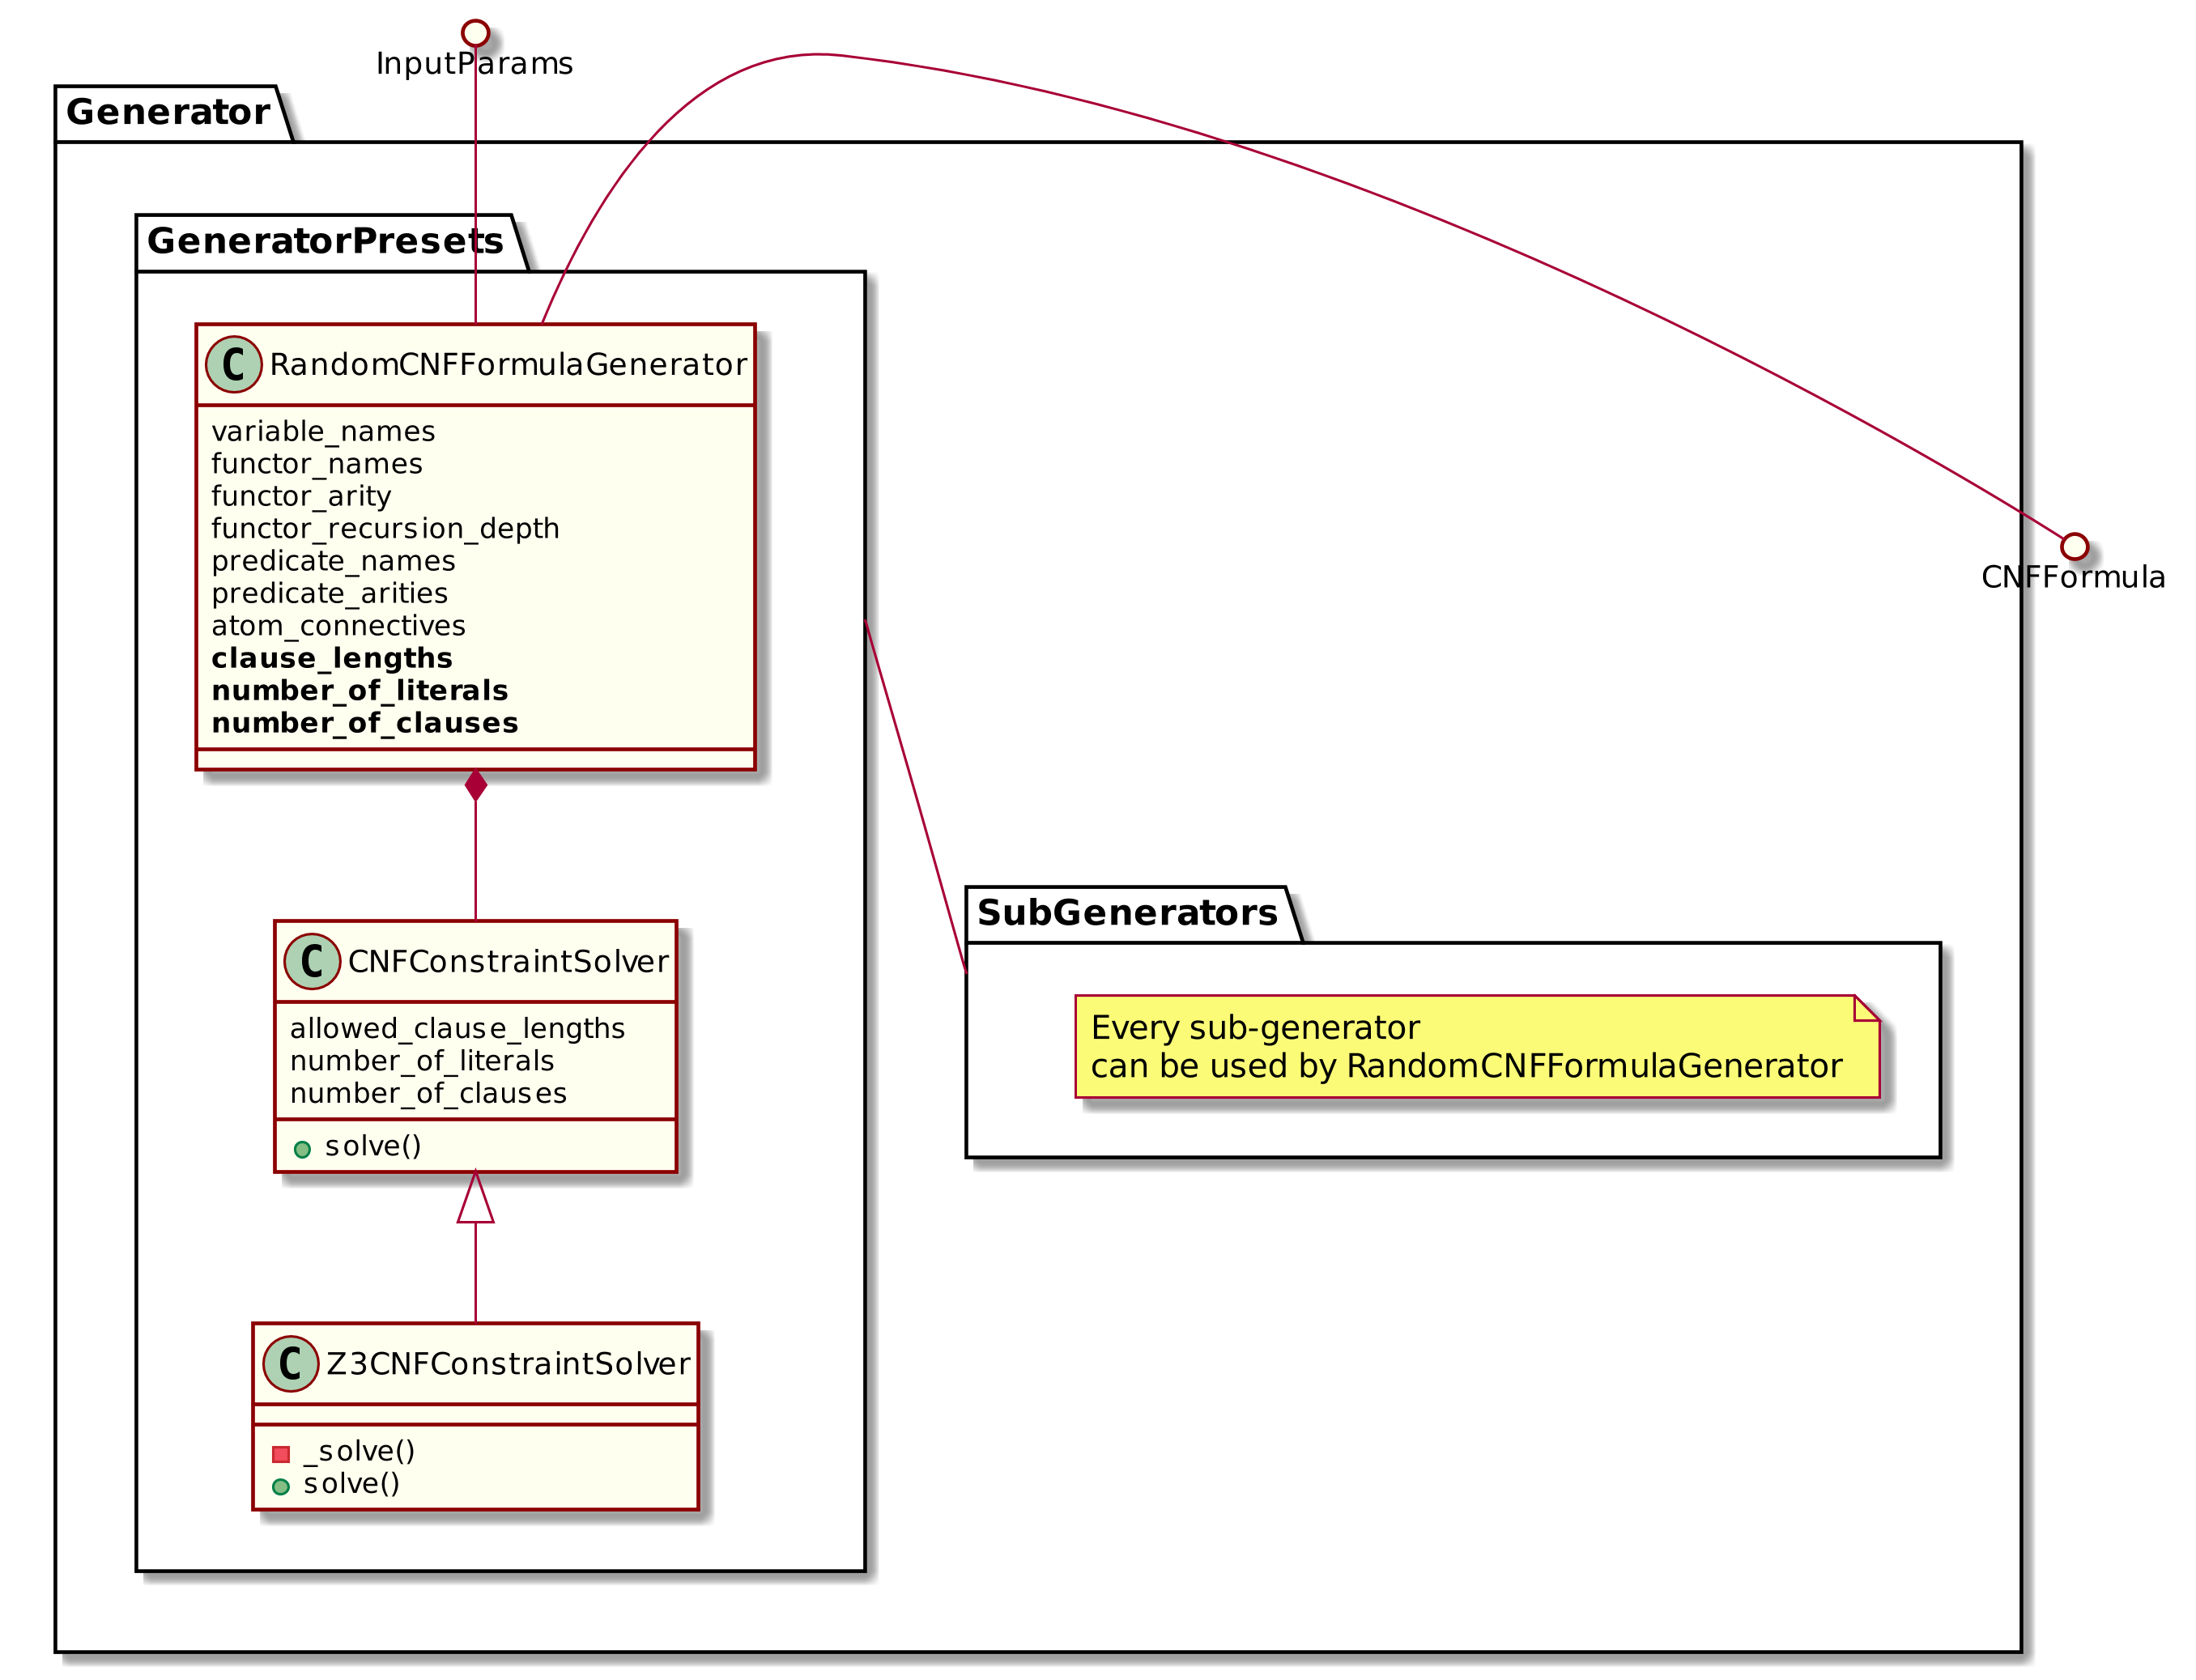
\includegraphics[width=\textwidth]{logic-formula-generator/cnf_formula_generator.png}
  \caption{Class diagram of CNF formula generator}
  \label{pic:cnf_generator_class_diagram}
\end{centering}
\end{figure}

\section{Export and generate statistics about formula}
\label{sec:GenerateStatisticsAboutFormula}

After generating formula it would be usefull to gather some information about it. 

\begin{figure}[h]
\begin{centering}
  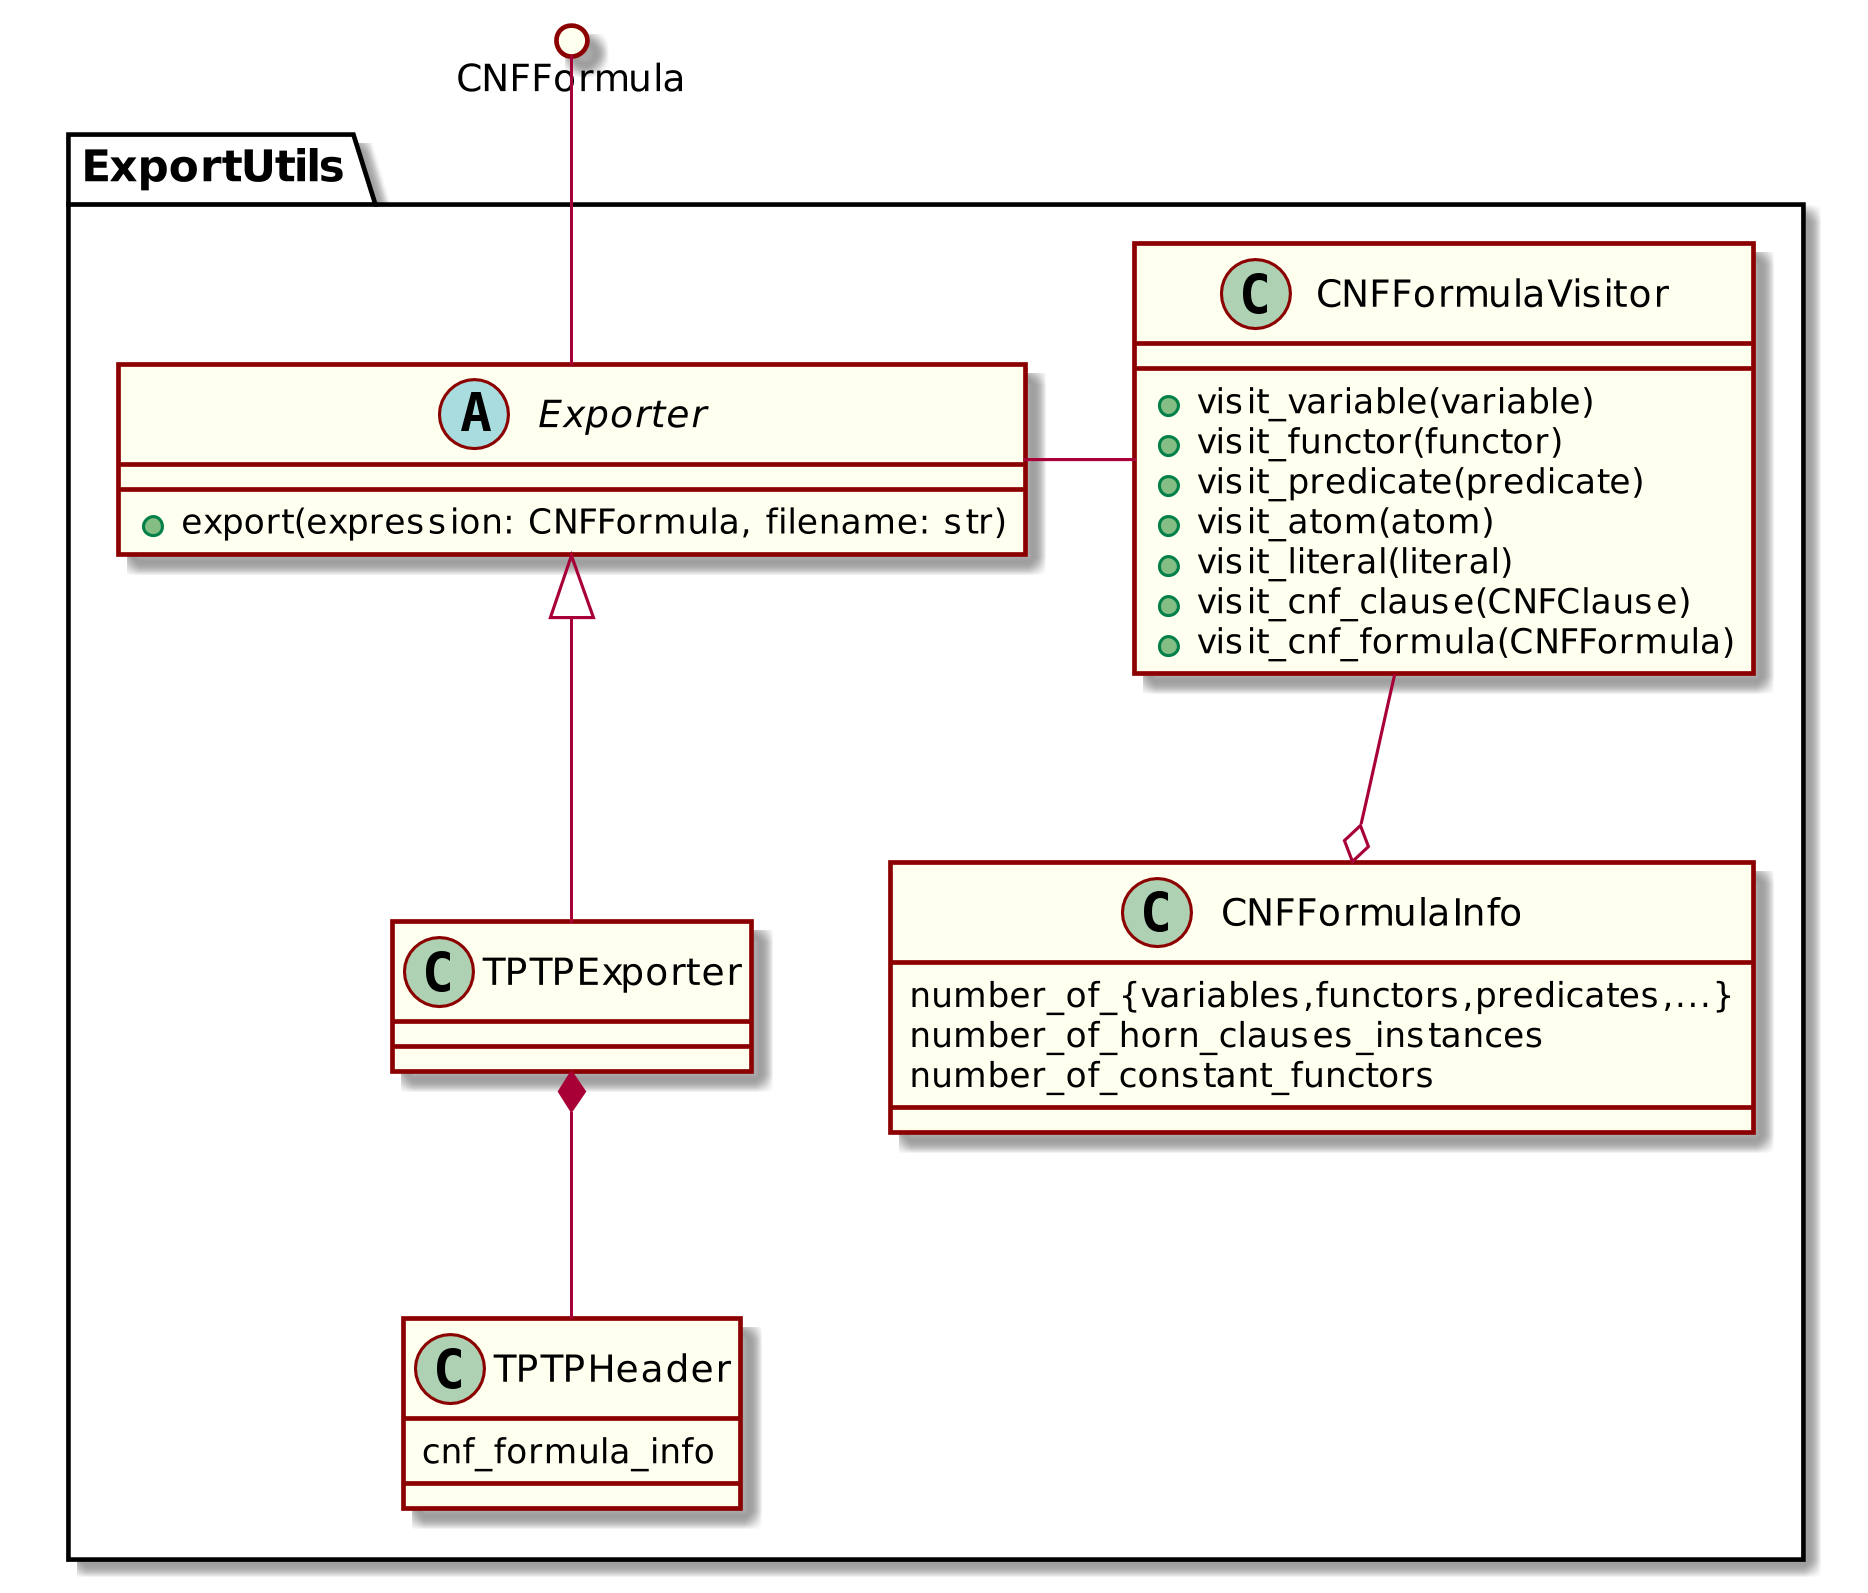
\includegraphics[width=\textwidth]{logic-formula-generator/fol/cnf_formula_statistics.png}
  \caption{Classes for which take part in generating statistics and exporting FOL CNF formula}
  \label{pic:CNFFormulaInfo}
\end{centering}
\end{figure}

\chapter{Generating random system properties}

One of the uses of random \gls{FOL} can be to generate random formula that represent system properties. That formula can be used as input for benchmark.

\section{Properties of computer systems}

System properties were first discussed in context of concurrency \cite{Lampert77} as a tool for formal verification multiprocess programs. One of first proposed properties were safety and liveness. These properties can apply to computer systems in general and be expressed in different formal systems.

\textbf{Liveness} \cite{Klimek99} is system property, that states, that something good will eventually happen.
Liveness formula guarantees that there is at least one case, where formula evaluates to true.

\textbf{Safety} \cite{Klimek99} is system property, that states, that something bad will never happens.
Safety formula must always be satisfied.

An informal example of system with liveness and safety properties could be an elevator. Statement: "Elevator will eventually stop" is liveness property of elevator as may be running now but eventually will hit the ceiling or floor. Statement: "Elevator must never run when the door is open" is safety property - the statement is always true.

\section{Properties of computer systems in first order logic}

In \gls{FOL} liveness and safety can be expressed as quantifiers, safety as universal quantifier and liveness as existential quantifier. 
If we were to use previously mentioned elevator example, the statements can be written as follows:

\begin{itemize}
  \item "Elevator will eventually stop" can be converted to logic formula: $\exists_t e(t)$ where predicate $e$ means "elevator is still", assuming $t<\infty$. The formula reads: there exists moment $t$ that the elevator is not moving
  \item "Elevator must never run when the door is open" can be converted to logic formula: $\forall_t \neg e(t) \land d(t)$ where predicate $e$ means "elevator is still" and $d$ means "doors are open". The formula reads: for every moment $t$ elevator is running and the doors are shut (at the same time).
\end{itemize}

\subsection{Properties of computer systems in first order logic in quantifier free}

Every \gls{FOL} can be converted to \gls{CNF}, so system properties can be also represented in \gls{CNF} but quantifiers must be also converted to CNF. The process of removing all the existential quantifiers from a formula is known as skolemization. The result is a formula in skolem normal form that is equivalent in computational complexity to the original. Skolemization follows several rules:


\begin{itemize}
  \item Variables bound by existential quantifiers which are not inside the scope of universal quantifiers can simply be replaced by constants - $\exists_t e(t)$ can be replaced by $e(f)$ where $f$ is new constant (functor)
  \item When the existential quantifier is inside a universal quantifier, the bound variable must be replaced by a Skolem function of the variables bound by universal quantifiers - $\forall_x  e(x) \land \exists_y e(t)$ can be replaced as $\forall_x e(x) \land e(f(x))$ 
\end{itemize}


Elevator example converted to quantifier free form looks as follows\footnote{removing quantifiers from first order logic can be automated with TPTP utility using TPTP2X utility, option \mintinline{text}{-t clausify:quaife}~\ref{sub:AdditionalToolsInTPTPLibrary} }::
\begin{itemize}
  \item "Elevator will eventually stop" $\exists_t e(t)$ in quantifier free form: $e(f)$ - new constant functor $f$ replaced variable $t$
  \item "Elevator must never run when the door is open" $\forall_t \neg e(t) \land d(t)$ in quantifier free form: $\neg e(X) \land d(Y)$ - 2 new variables $X$ and $Y$ replaced variable $t$ bounded to universal quantifier
\end{itemize}

In conclusion safety and liveness can be represented in CNF as 2 form of predicates: liveness as predicate, where arguments are only constant functors, safety as predicate where arguments are variables.

\section{Dataset with system properties}

The goal is to generate liveness and safety clauses, but do not mix them. In order to achieve that, class $PredicateGenerator$ needs to be modified to yield either formulas with all variables (safety) or formulas with 0-arity functor (liveness). To achieve that $PredicateGenerator$ was subclassed and used to create alternative version of $CNFFormulaGenerator$.

\begin{figure}[H]
\begin{centering}
  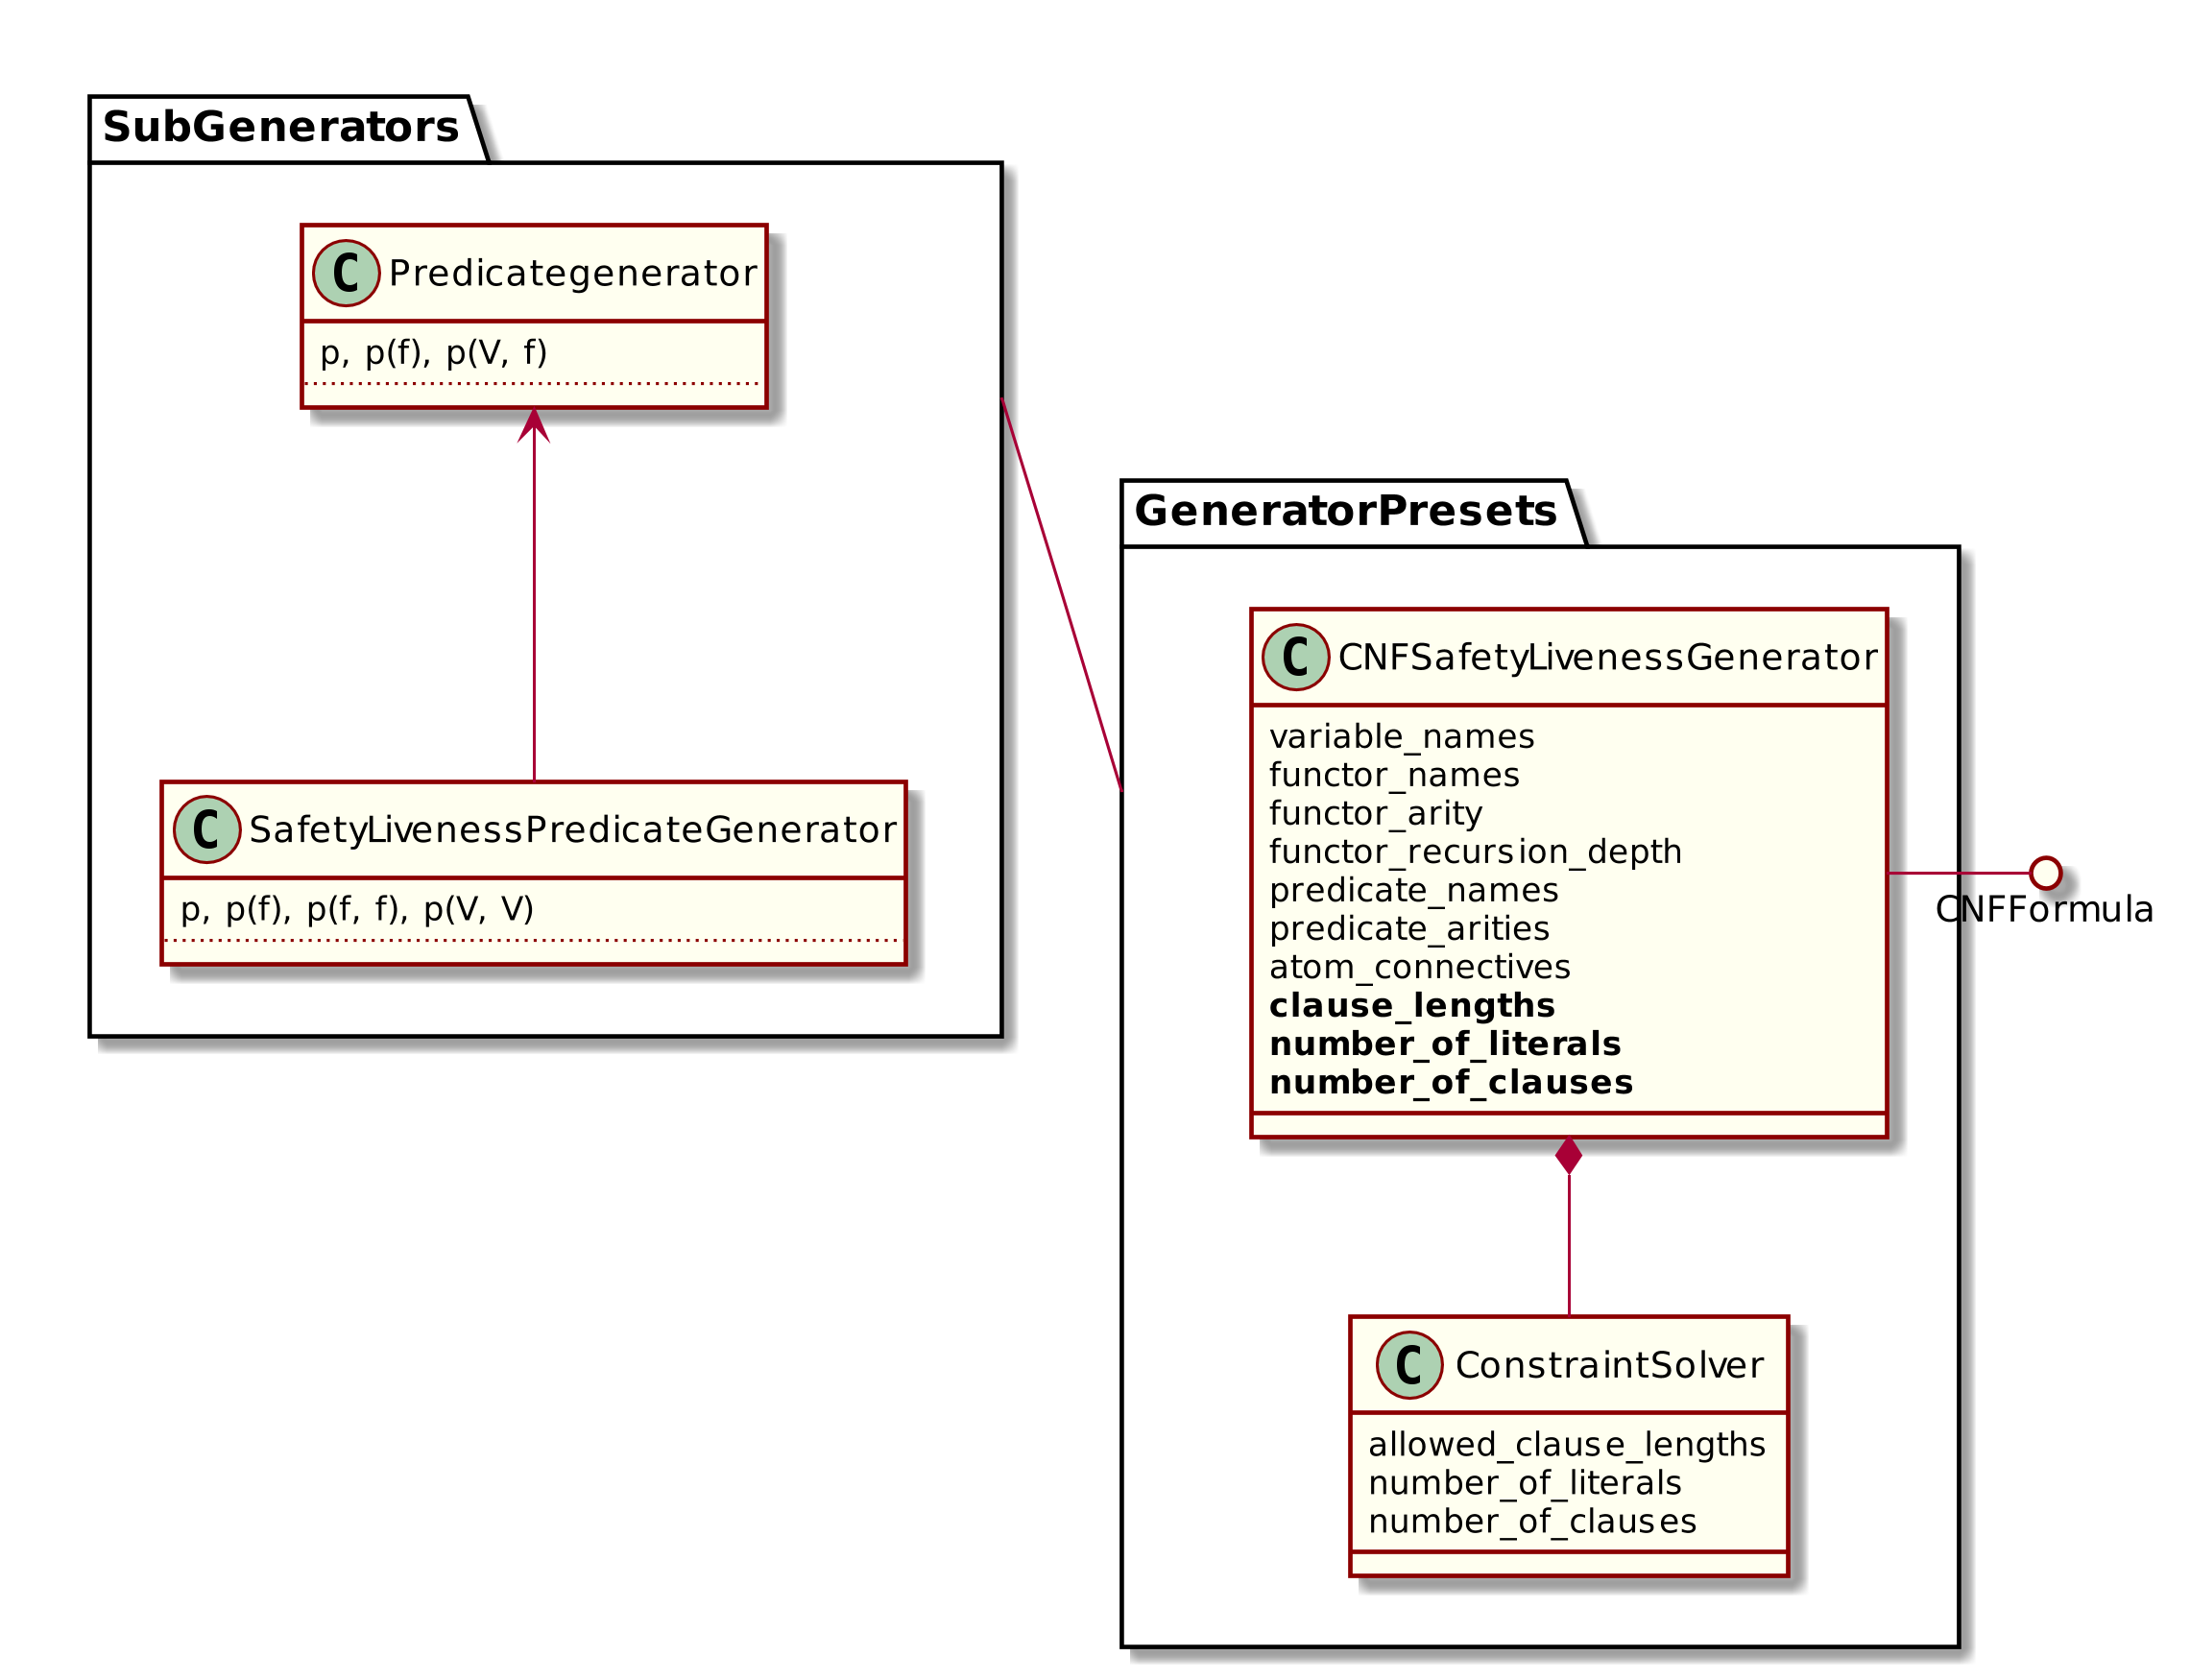
\includegraphics[width=\textwidth]{logic-formula-generator/fol/safety_liveness_predicate_generator.png}
  \caption{Subclassed PredicateGenerator mimics safety and liveness formulas}
\end{centering}
\end{figure}

In this study the impact of ratio of number of atoms to number of clauses will be presented.
Formulas with 1000 atoms and 100, 200, 300, 400, 500 clauses were generated, 50 for each combination, 250 in total. 50 formulas is rather small sample to reason about, but it was chosen because of time and hardware limitations. Number of atoms and number of clauses can vary within 5\%, although solver tends to yield small numbers first in general. The rest of parameters for formulas is shown in listing~\ref{lis:CNFSafetyLivenesSnippet}.

\subsection{Results}

Formulas were generated and were benchmarked against solvers Prover9 and SPASS. Results are shown in picture~\ref{pic:SPASSProverNumberOfClauses} and~\ref{pic:SPASSProverMemory}. Maximum execution time of single formula was trimmed at 300 seconds. 

First thing worth noting is SPASS solver is capable of solving much more formulas than Prover9. SPASS uses somewhat constant memory whereas Prover9 requires more memory the longer it runs.

It can be said that formulas with ratio atoms to clauses below 4 can be considered easy, as all of them were solved by both solvers.

\begin{listing}[ht]
  \caption{Snippet for generating dataset of safety and liveness formulas}
  \label{lis:CNFSafetyLivenesSnippet}
\begin{minted}{python}
gen = CNFSafetyLivenessGenerator(
    variable_names={f'V{i}' for i in range(10)},
    functor_names={f'f{i}' for i in range(20)}, functor_arity={0},
    functor_recursion_depth=0,
    predicate_names={f'p{i}' for i in range(20)}, predicate_arities={i for i in range(5)},
    atom_connectives={''},
    clause_lengths={i for i in range(2, 11)},
    number_of_clauses=IntegerRange.from_relative(number_of_clauses, threshold),
    number_of_literals=IntegerRange.from_relative(number_of_literals, threshold),
    literal_negation_chance=0.1,
)
\end{minted}
\end{listing}

\begin{listing}[H]
  \caption{Example of generated formula (limited)}
\begin{tptpcode}
% ----------------------------------------------------------------------------
% File      : 0.p 
% Syntax    : Number of clauses     :   95 ( 95 non-Horn;   0 unit;   - RR)
%             Number of atoms       :  950 (  0 equality)
%             Maximal clause size   :   10 ( 10 average)
%             Number of predicates  :   20 (206 propositional; 0-4 arity)
%             Number of functors    :   20 (940 constant;   0 arity)
%             Number of variables   :  943 (327 singleton)
%             Maximal term depth    :    0 (  - average)
% 
% ----------------------------------------------------------------------------
cnf(name,axiom,p4(V6)|p10(V1, V4, V9)|~p7|p17|p1(V4, V3, V9)|p7|p17|p1(f11, f11, f5)|p7|~p0(f2)).
cnf(name,axiom,p2(V7, V9)|p4(f19)|p2(f8, f5)|p10(f7, f8, f8)|p12|p6(V2, V6)|p14(f8, f16, f9, f16)|p3(f14, f3, f14, f18)|p11(V3, V9)|p12).
...
\end{tptpcode}
  \label{lis:TPTPExample}
\end{listing}

\newpage

\begin{figure}[H]
\centering
  \begin{subfigure}{0.8\textwidth}
\centering
  \includegraphics[width=\textwidth]{"logic-formula-generator/dataset_analysis/cnf charts/01 Prover9 number of clauses vs time".jpg}
  \label{pic:benchmark_results}
  \end{subfigure}

  \begin{subfigure}{\textwidth}
\centering
  \includegraphics[width=\textwidth]{"logic-formula-generator/dataset_analysis/cnf charts/11 SPASS number of clauses vs time".jpg}
  \end{subfigure}
  \caption{On left axis time of execution is presented (300s is max), marked with blue. On right axis ratio clauses to atoms is presented. Ratio 2 means there are 2 atoms for each clause}
  \label{pic:SPASSProverNumberOfClauses}
\end{figure}

\begin{figure}[H]
\centering
  \begin{subfigure}{0.8\textwidth}
\centering
  \includegraphics[width=\textwidth]{"logic-formula-generator/dataset_analysis/cnf charts/02 Prover9 number of clauses vs peak memory".jpg}
  \label{pic:benchmark_results}
  \end{subfigure}

  \begin{subfigure}{\textwidth}
\centering
\includegraphics[width=\textwidth]{"logic-formula-generator/dataset_analysis/cnf charts/12 SPASS number of clauses vs peak memory".jpg}
  \end{subfigure}
  \caption{On left axis peak RAM memory is presented, marked with blue. On right axis ratio clauses to atoms is presented. Ratio 2 means there are 2 atoms for each clause}
  \label{pic:SPASSProverMemory}
\end{figure}

% \section{Modified dataset}
%
% TODO
%
% \begin{figure}[H]
% \begin{centering}
%   \includegraphics[width=\textwidth]{"logic-formula-generator/fol/safety_liveness_predicate_generator_1_in_10".png}
%   \caption{Subclassed PredicateGenerator mimics safety and liveness formulas}
% \end{centering}
% \end{figure}
%
% \subsection{Results}
%
% TODO
%
% Charts are only placeholders:

% \newpage
%
% \begin{figure}[H]
% \centering
%   \begin{subfigure}{0.8\textwidth}
% \centering
%   \includegraphics[width=\textwidth]{"logic-formula-generator/dataset_analysis/cnf charts/01 Prover9 number of clauses vs time".jpg}
%   % \label{pic:}
%   \end{subfigure}
%
%   \begin{subfigure}{\textwidth}
% \centering
%   \includegraphics[width=\textwidth]{"logic-formula-generator/dataset_analysis/cnf charts/11 SPASS number of clauses vs time".jpg}
%   \end{subfigure}
%   \caption{On left axis time of execution is presented (300s is max), marked with blue. On right axis ratio clauses to atoms is presented. Ratio 2 means there are 2 atoms for each clause}
%   % \label{pic:}
% \end{figure}
%
% \begin{figure}[H]
% \centering
%   \begin{subfigure}{0.8\textwidth}
% \centering
%   \includegraphics[width=\textwidth]{"logic-formula-generator/dataset_analysis/cnf charts/02 Prover9 number of clauses vs peak memory".jpg}
%   % \label{pic:}
%   \end{subfigure}
%
%   \begin{subfigure}{\textwidth}
% \centering
% \includegraphics[width=\textwidth]{"logic-formula-generator/dataset_analysis/cnf charts/12 SPASS number of clauses vs peak memory".jpg}
%   \end{subfigure}
%   \caption{On left axis peak RAM memory is presented, marked with blue. On right axis ratio clauses to atoms is presented. Ratio 2 means there are 2 atoms for each clause}
%   % \label{pic:}
% \end{figure}
%

\chapter{Conclusion}

In this thesis a base for random first order logic formula generator has been presented. The generator can be easily extended for user specific needs. For example user can add arbitrary rule (by inheriting one of generators) that elements must follow during generation, more output formats can be added.
Presented solution can be extended to follow constraints related to any other \gls{FOL} element like limited number of variables, functors and so on.
The biggest challenge in described solution is randomizing solutions from constraint solver. Solving user constrains is problem of integer programming (NP problem) that is why enumerating them all is not an option. Instead random number of solutions is skipped to preserve at least pseudo-randomness.

Alternative approach to using \gls{SMT} solver would be to take locally optimal decisions and introduce some randomness when taking those decisions. This approach would create arguably "more" random result but introduces number of drawbacks:

\begin{itemize}
  \item taking many local decisions may not be faster than taking one global - that requires in depth analysis,
  \item this is non deterministic approach - some possible variants of formula might never/rarely be reached, one can argue if it is even possible to create such algorithm
  \item adding new constraint would be much more complicated
\end{itemize}

The future development of presented generator would allow to generate formulas in different normal forms, more readable suggestions for constrains errors and ability to auto correct user constraints errors.



% itd.
% \appendix
% \include{dodatekA}
% \include{dodatekB}
% itd.

\printglossary

\printbibliography

\end{document}
